% !TEX root = main.tex
\section{Experiments and Results}


\begin{table}[t]
    \begin{center}
    \setlength{\tabcolsep}{1.3mm}
\begin{tabular}{r|cccccccccc}
\hline
& {\bf PDIA } & PDIA-MAP & PDIA-$\beta=0$ & HMM & 2-gram& 3-gram & 4-gram & 5-gram & 6-gram & SM \\
\hline
AIW & 2.25 & 2.64 & 2.25 & 2.98 & 3.29 & 2.73 & 2.45 & 2.38 & 2.35 &\\
DNA & 1.893 & 1.906 & 1.893 & 1.909 & 1.915 & 1.908 & 1.905 & 1.903 & 1.910 & \\
\hline
\hline
AIW & 205.1 & 212 & 203.8 & 52 & 28 & 382 & 2023 & 5592 & 10838 &\\
DNA & 46.0 & 49 & 46.2 & 95 & 5 & 21 & 85 & 341 & 1365 & \\
\hline
\end{tabular}
\end{center}
\caption[Short]{Benchmark performance of PDIA inference algorithms versus standard sequence models.}
\label{table:results}
\end{table}

\begin{figure}[htbp]
\begin{center}
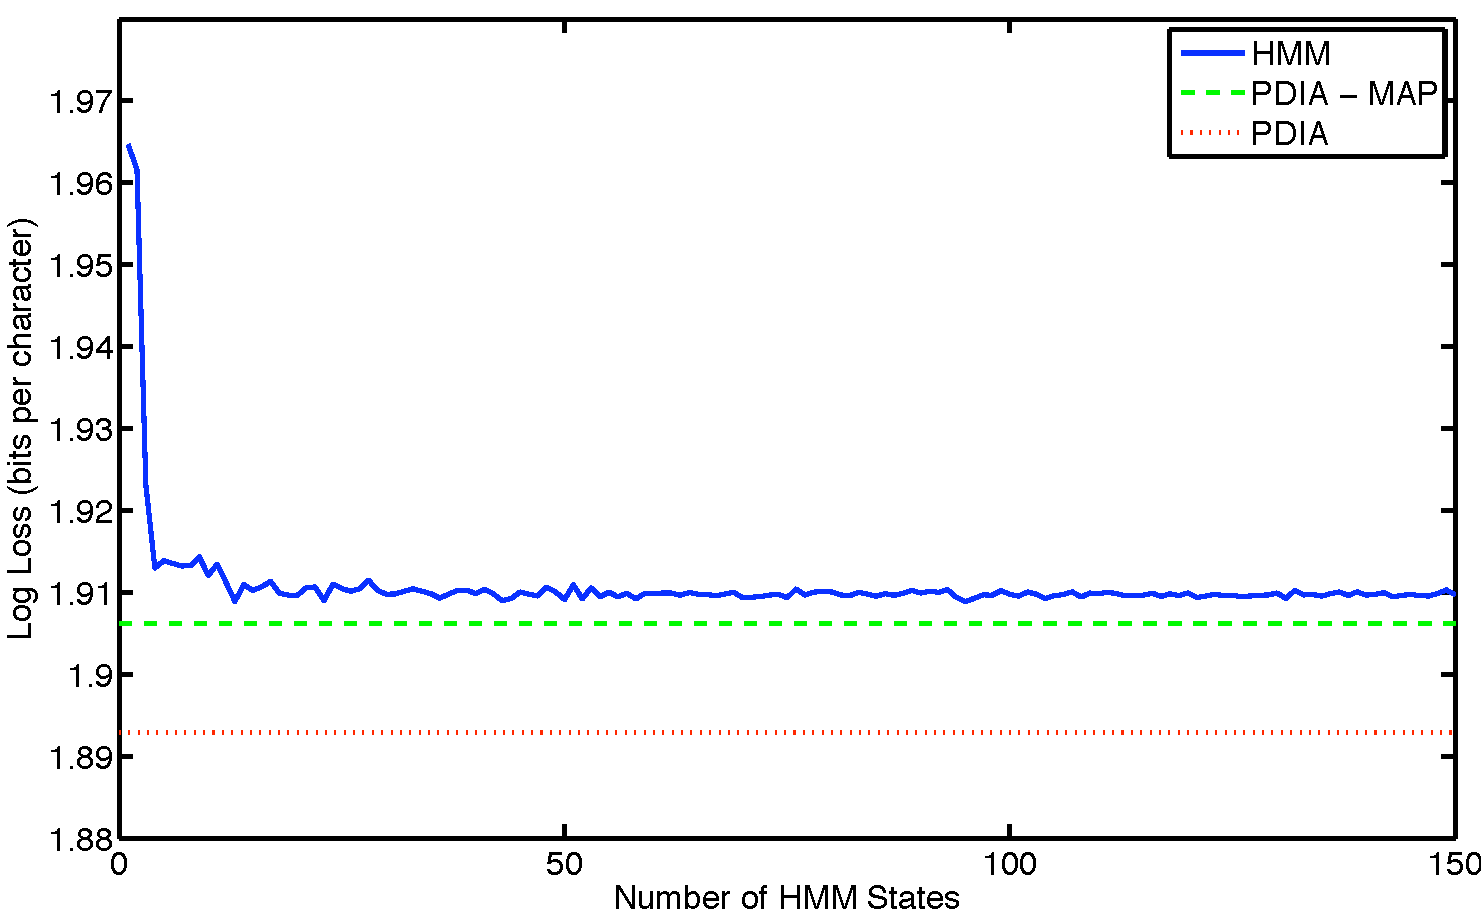
\includegraphics[width=10cm]{results/dna_hmm}
\caption{DNA HMM EM Baseline}
\label{fig:dna_hmm}
\end{center}
\end{figure}


\begin{figure}[htbp]
\begin{center}
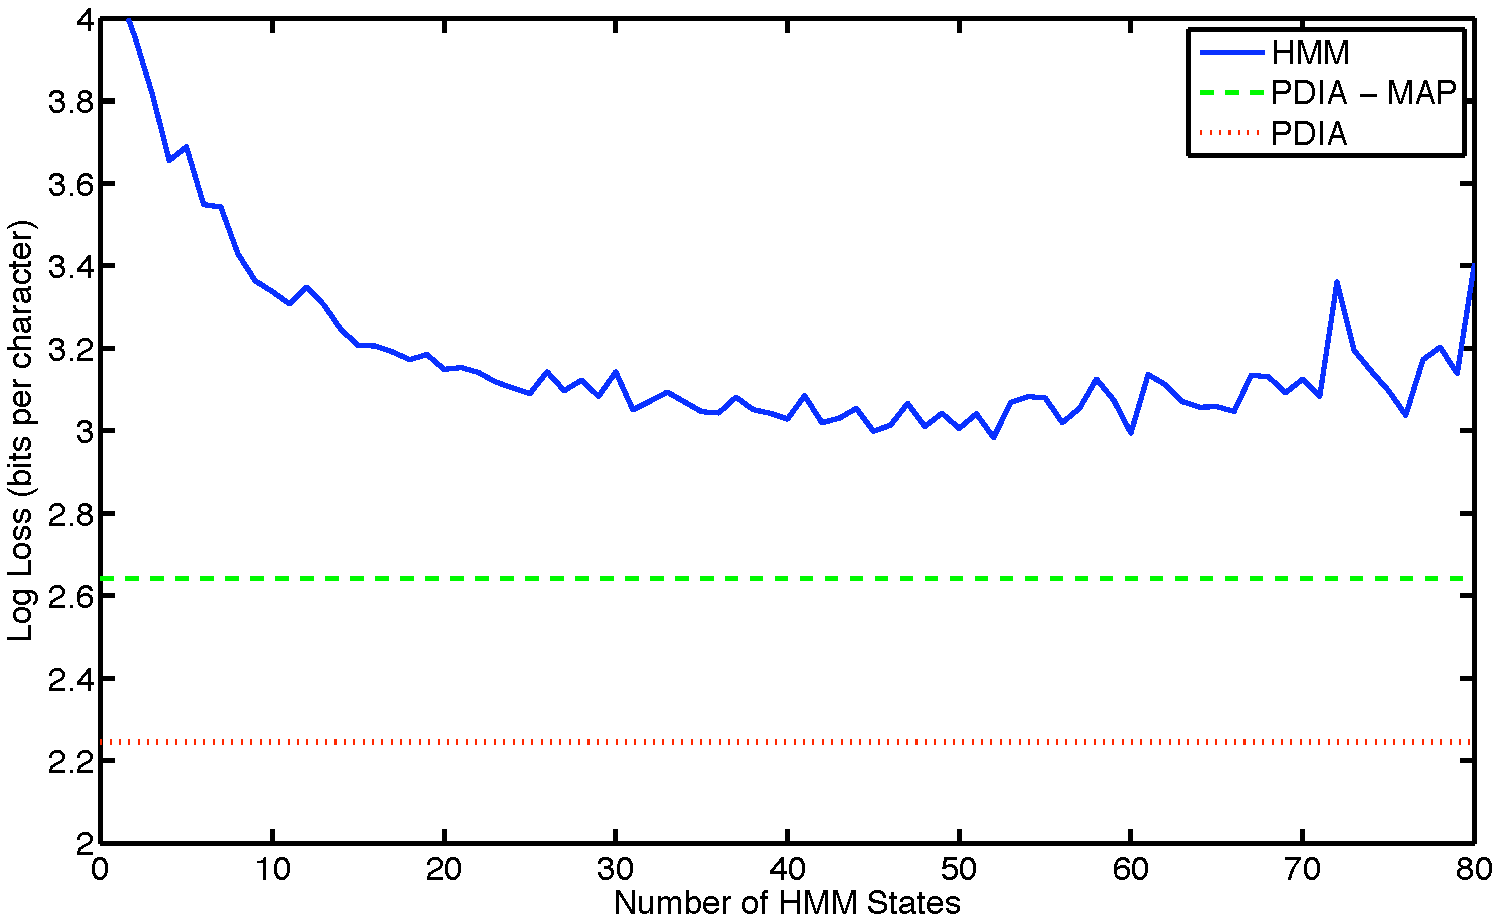
\includegraphics[width=10cm]{results/aiw_small_hmm}
\caption{AIW HMM EM Baseline}
\label{fig:aiw_small_hmm}
\end{center}
\end{figure}

\begin{figure}[htbp]
\begin{center}
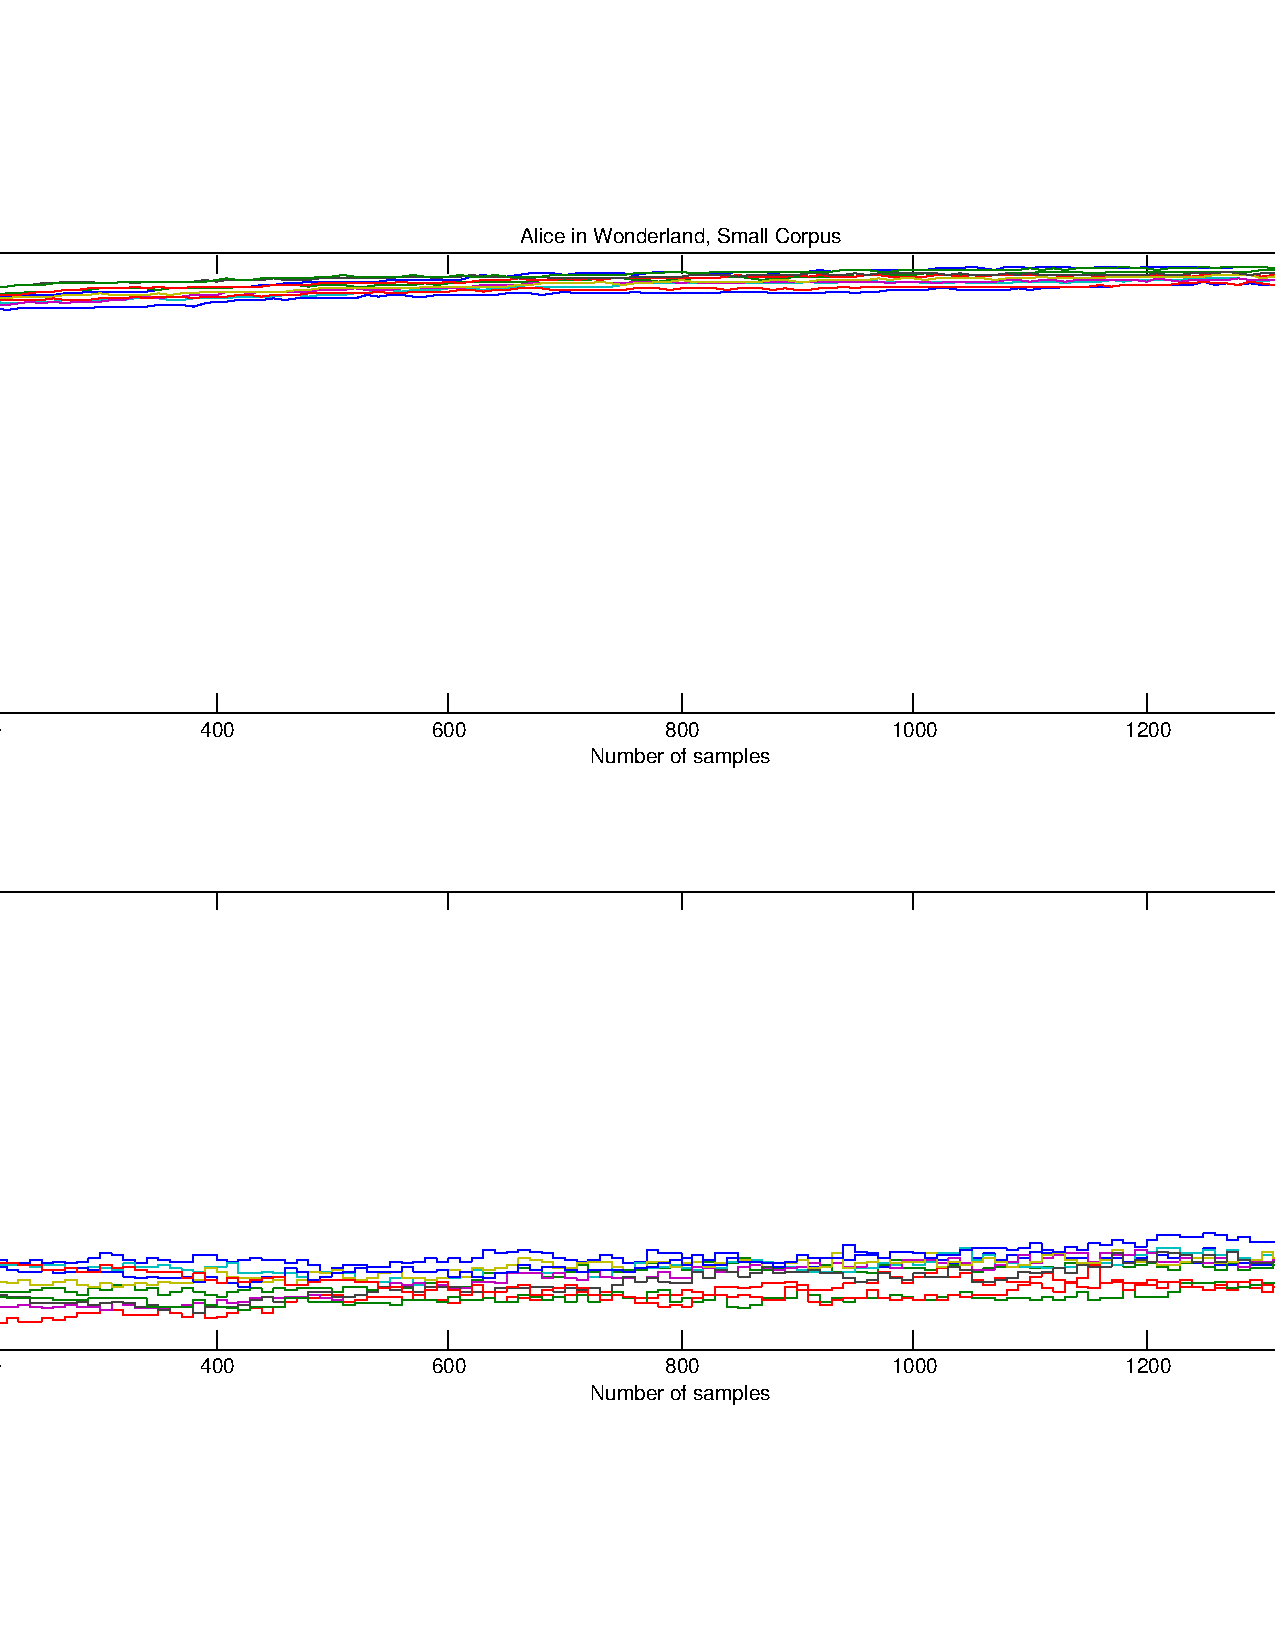
\includegraphics[width=5cm]{results/aiw_small_sampler_trace}
\caption{AIW small sampler trace }
\label{fig:aiw_small_sampler_trace}
\end{center}
\end{figure}

\begin{figure}[htbp]
\begin{center}
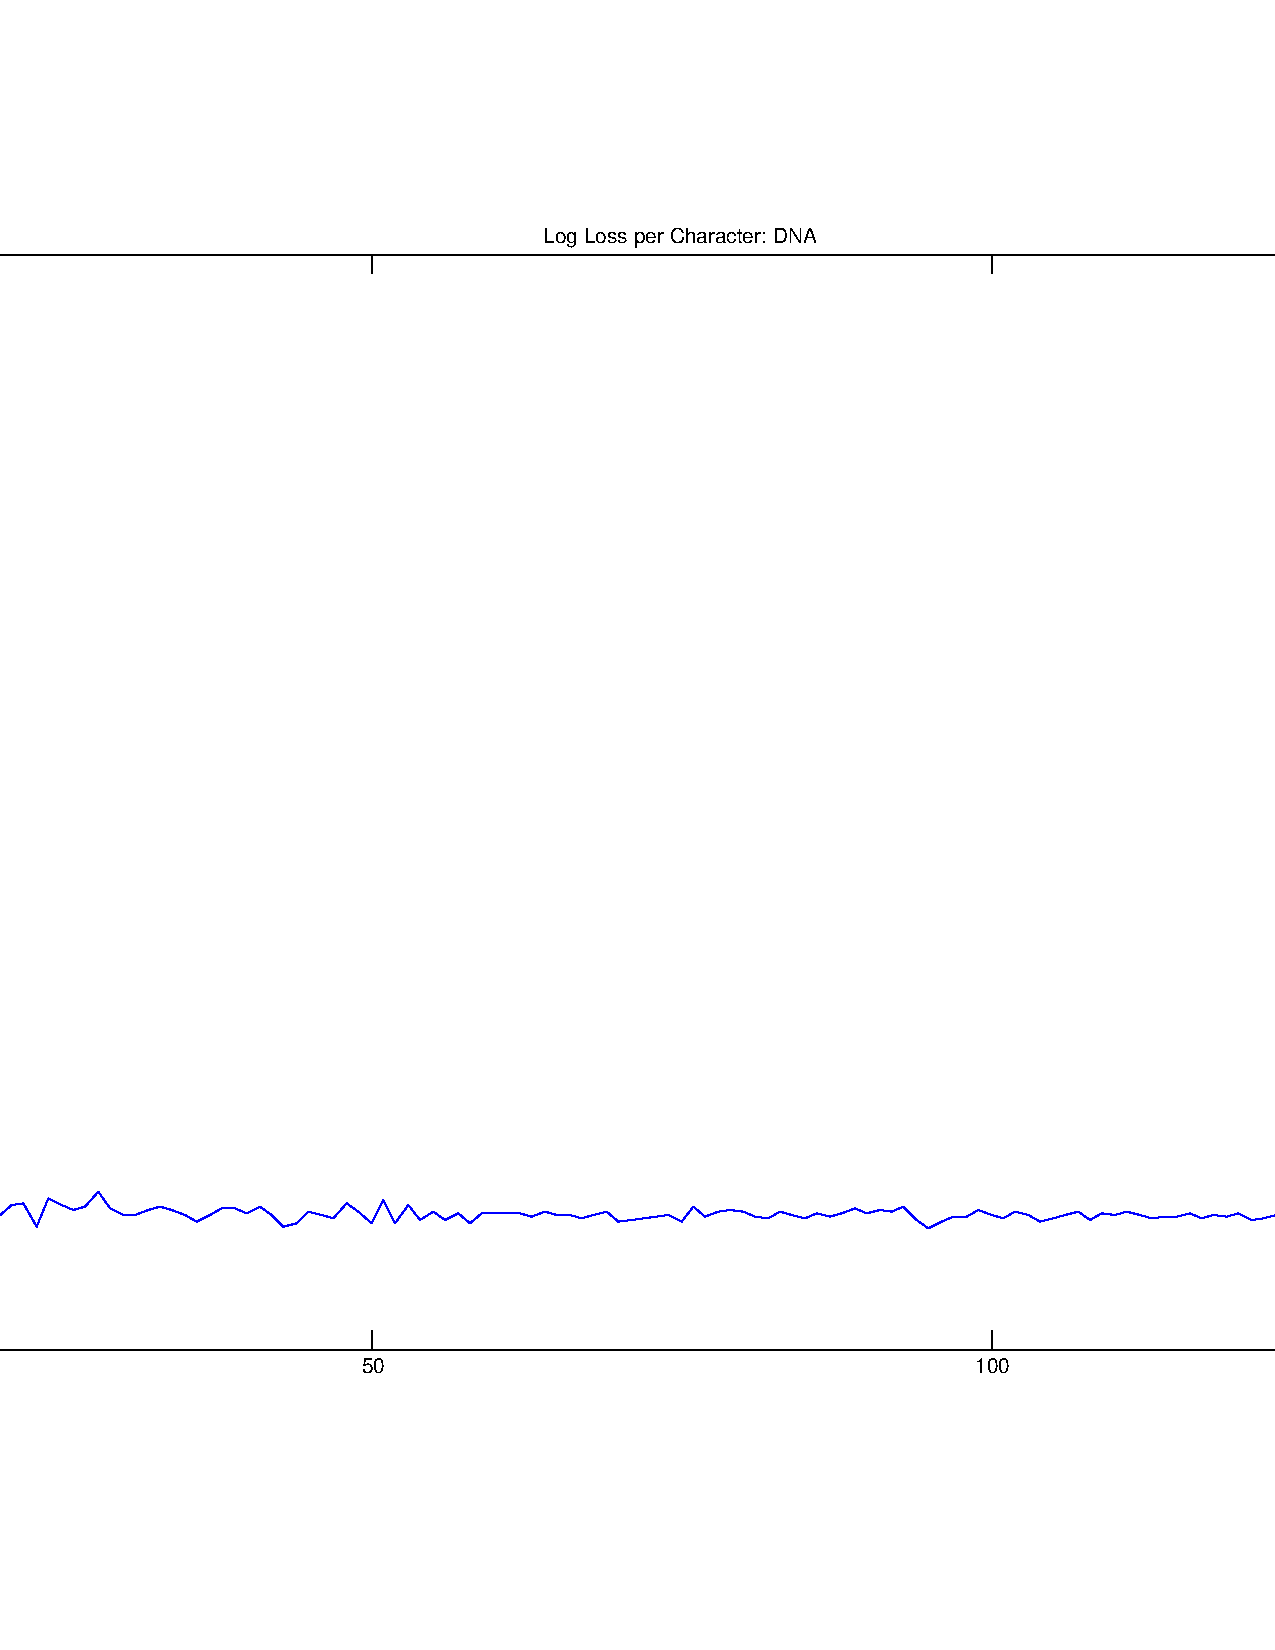
\includegraphics[width=5cm]{results/dna_hmm_baseline}
\caption{DNA EM }
\label{fig:dna_hmm_baseline}
\end{center}
\end{figure}


We ran the PDIA on two datasets: Alice in Wonderland and mouse DNA.  Alice in Wonderland was preprocessed to remove all non-alphabetic characters, shift upper case to lower case, and split along sentence dividers to yield a 27-character alphabet (a-z and space) and 1639 sentences with a total of 132794 characters.  We used the first 1200 sentences (100210 characters) to train the model and the rest to test.  For some experiments we also used a smaller subset of Alice in Wonderland consisting of 100 randomly chosen training sentences (9986 characters) and 50 random test sentences (3891 characters).  The mouse DNA dataset consists of a fragment of chromosome 2 with 194173 base pairs, which we treated as a single unbroken string.  We used the first 150000 base pairs for training and the rest for testing.  For Alice in Wonderland, the state of the model was always set to $q_0$ at the start of a string.  For DNA, the state of the model at the start of the test data was set to the last state of the model on the training data.

When testing the predictive performance of a trained model, we sometimes encountered symbol/state pairs that were not seen in the training data.  In these cases we sampled a new element of the transition matrix from the CRF, as described in \ref{sec:BPDFAs}.  We averaged the probability of each character over multiple trials in this case, to best approximate the true predictive probability with those elements of the transition matrix integrated out.